\subsection{ROLLO: Reactor evOLutionary aLgorithm Optimizer}
\begin{frame}
    \frametitle{ROLLO: Reactor evOLutionary aLgorithm Optimizer}
    \begin{figure}
        
\includegraphics[width=0.7\linewidth]{figures/rollo-logo.png} 
        \caption{ROLLO (Reactor evOLutionary aLgorithm Optimizer) logo.}
    \end{figure}
    \begin{itemize}
        \item ROLLO (Reactor evOLutionary aLgorithm Optimizer) is a Python package 
        that applies evolutionary algorithms to optimize nuclear reactor design
        \item ROLLO provides a general genetic algorithm framework, sets up 
        parallelization for the user, and promotes usability with an input file that
        only exposes mandatory parameters
        \item Design Goals: effective, flexible, open-source, parallel,
        reproducible
    \end{itemize}
\end{frame}

\begin{frame}
    \frametitle{How does ROLLO work?}
    \begin{minipage}[c]{0.45\textwidth}
        \begin{itemize}
            \item Reads and validates the JSON input file
            \item Initializes the \acrfull{DEAP} genetic algorithm hyperparameters and 
            operators 
            \item Runs the genetic algorithm  
            \item During the run, nuclear software evaluates each individual reactor 
            model's fitness
        \end{itemize}
    \end{minipage}\hfill
    \begin{minipage}[c]{0.52\textwidth}
        \centering
        \begin{figure}
            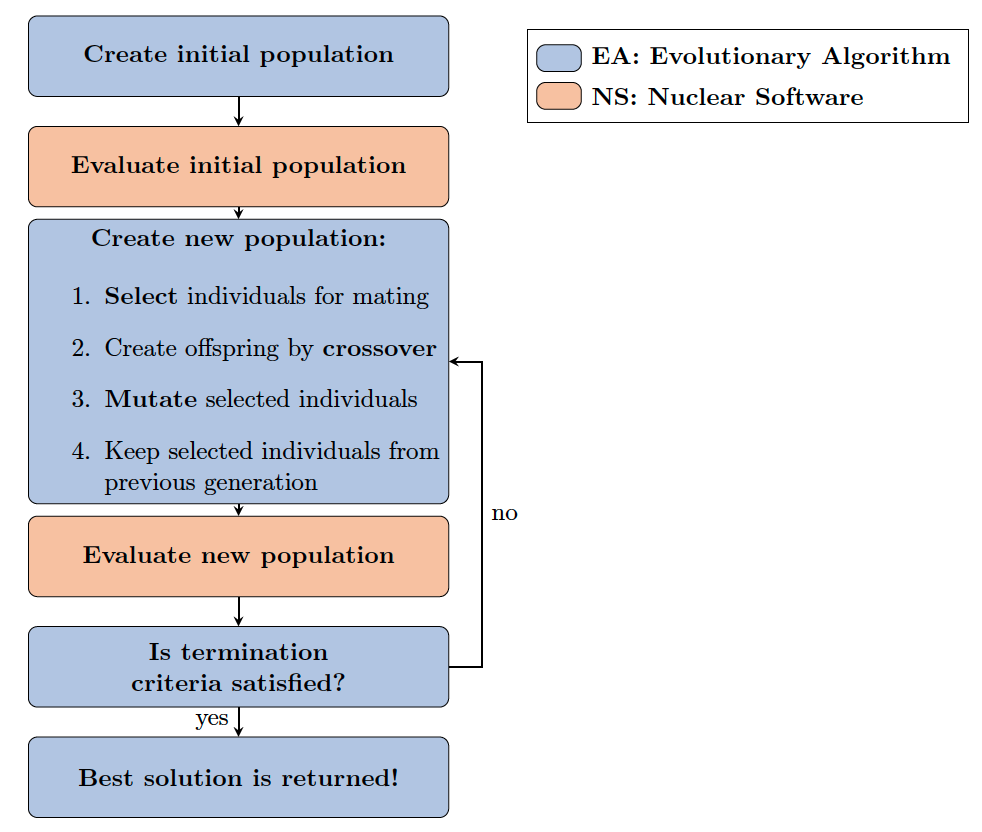
\includegraphics[width=\linewidth]{figures/rollo-flow.png} 
            \caption{ROLLO Genetic Algorithm Flow.}
        \end{figure}
    \end{minipage}
\end{frame}

\begin{frame}
    \frametitle{ROLLO $^{239}Pu$ Critical Bare Sphere Input File}
    \begin{figure}
        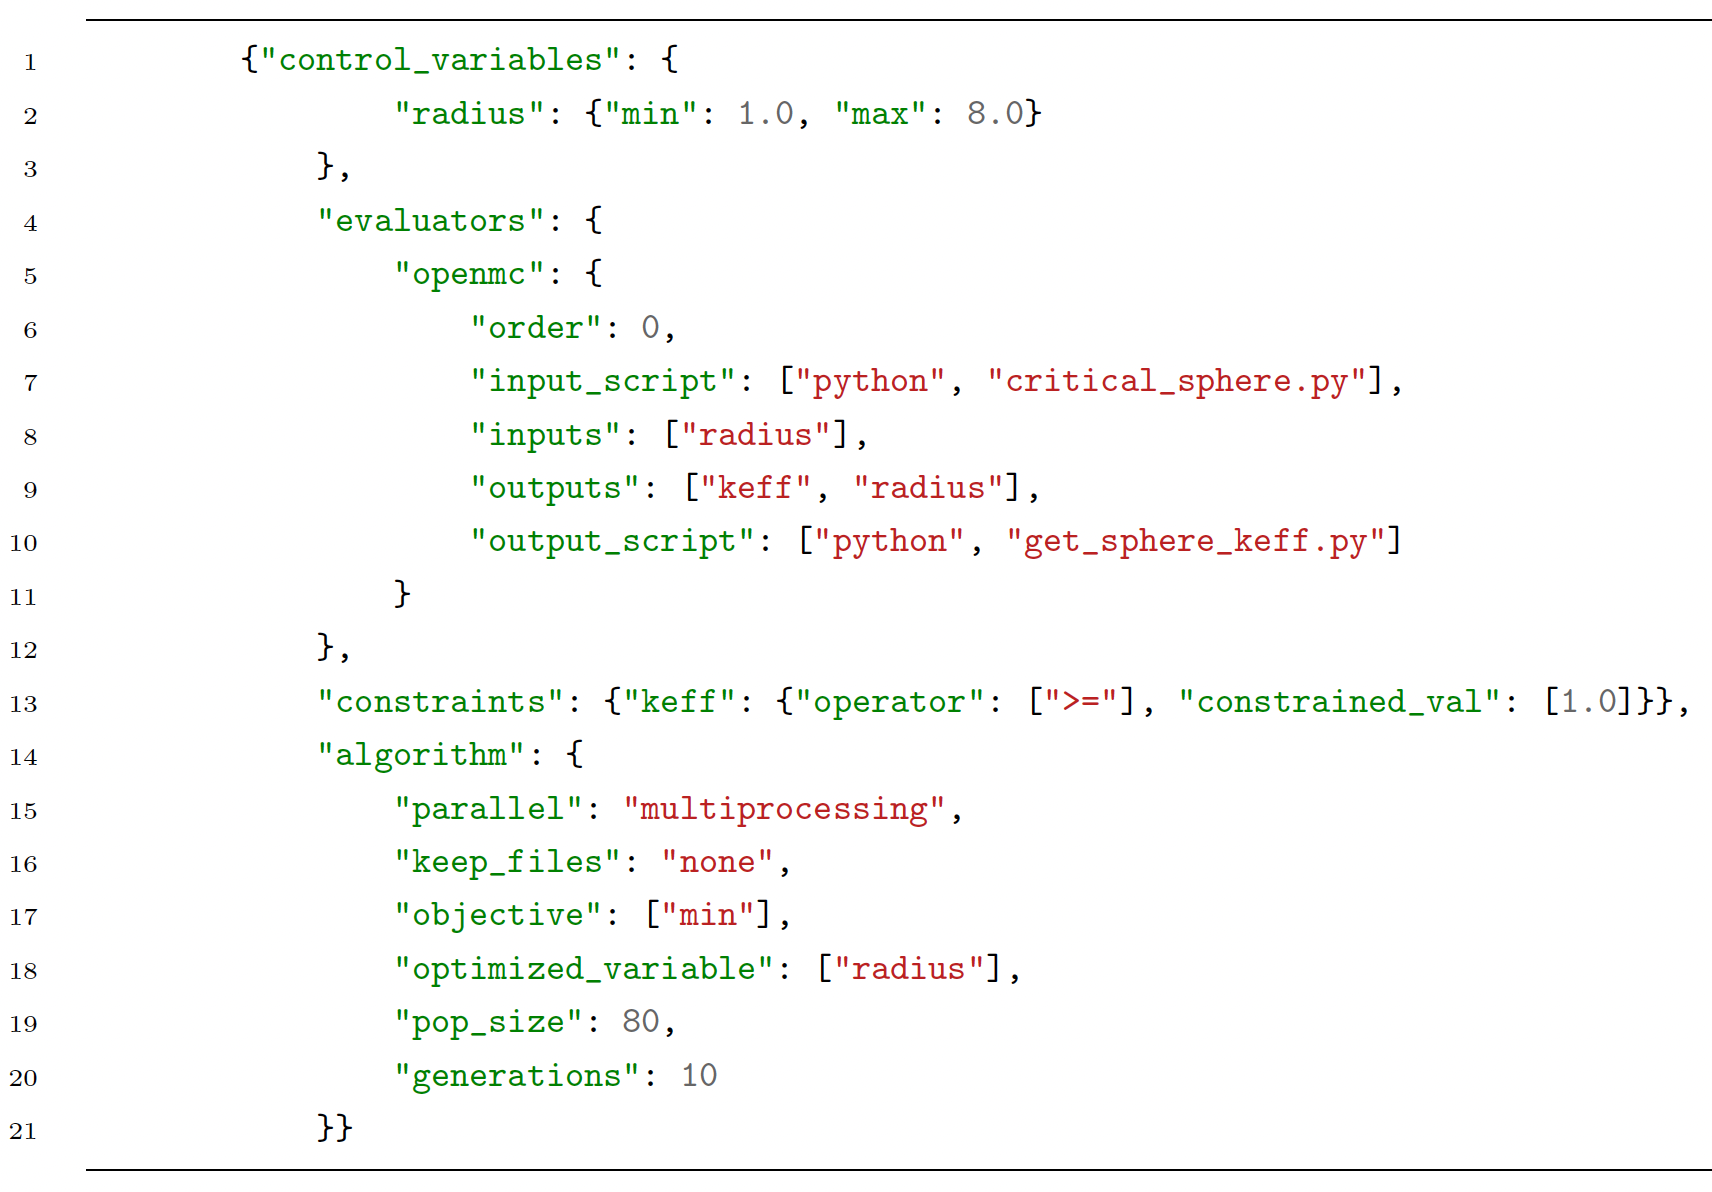
\includegraphics[width=0.49\linewidth]{figures/rollo-verify-file.png} 
        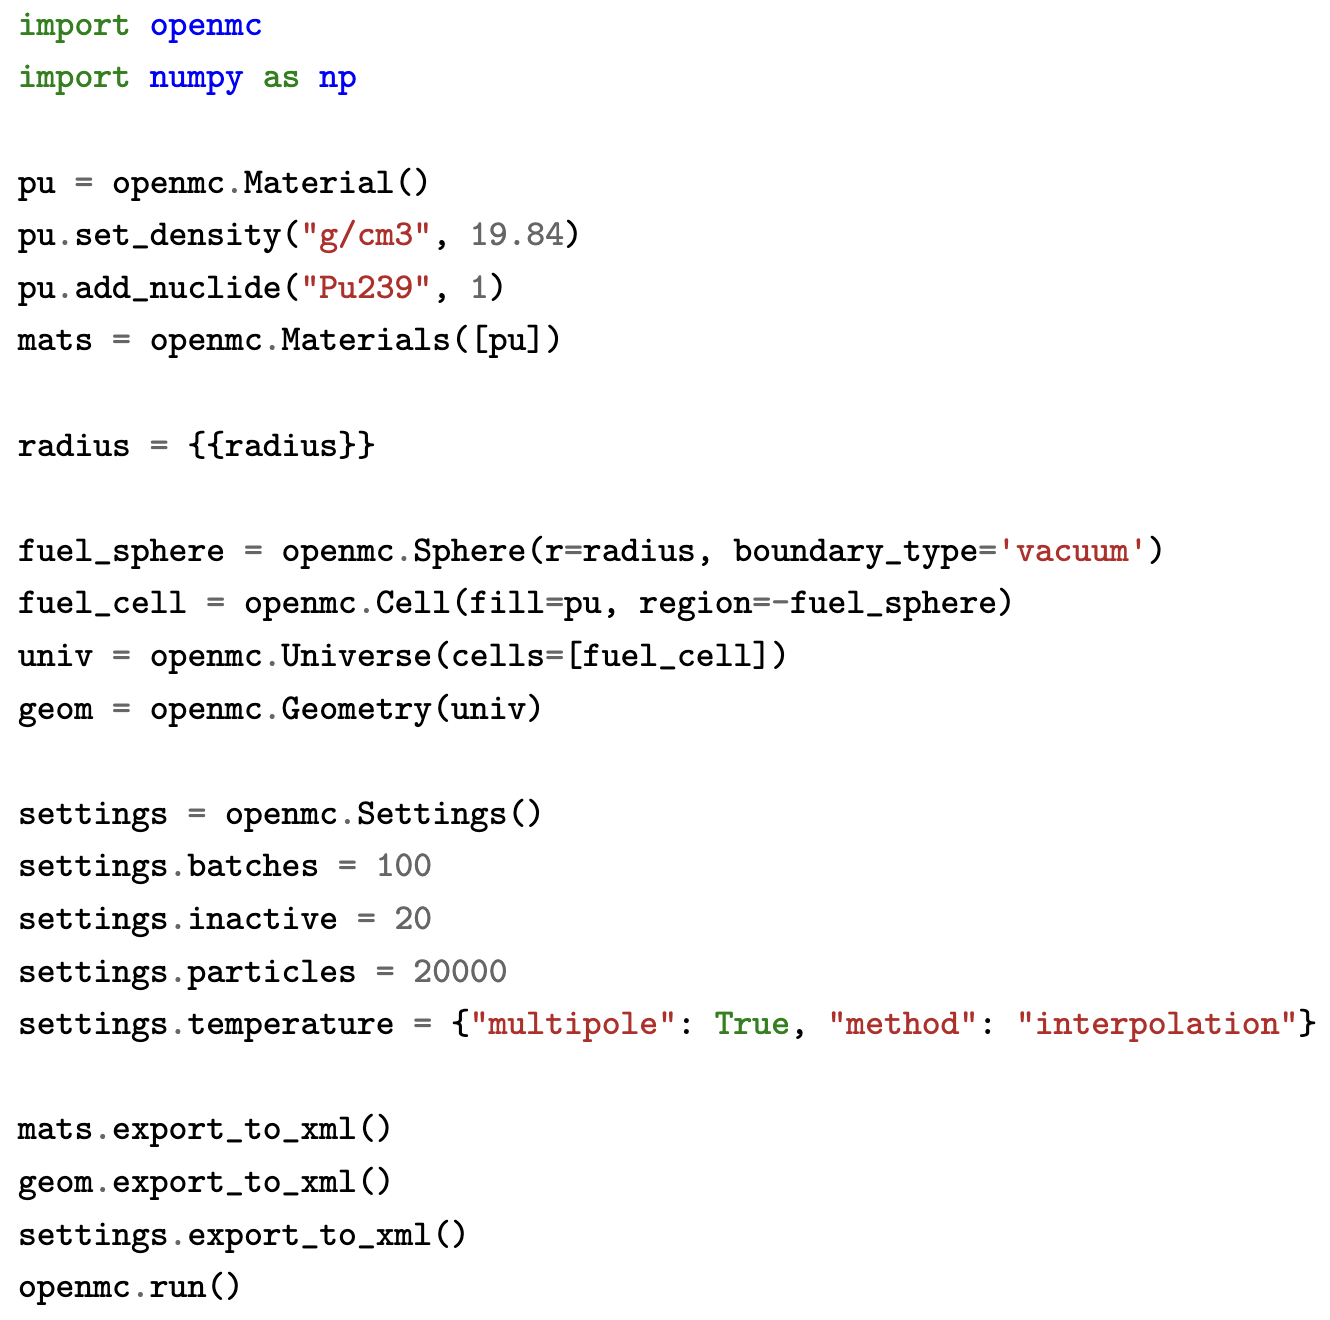
\includegraphics[width=0.49\linewidth]{figures/rollo-verify-file2.png}
        \caption{ROLLO $^{239}Pu$ Critical Bare Sphere Input File.}
    \end{figure}
\end{frame}

\subsection{ROLLO Verification}
\begin{frame}
    \frametitle{ROLLO Successfully Verified with $^{239}Pu$ Critical Bare Sphere}
    \begin{figure}
        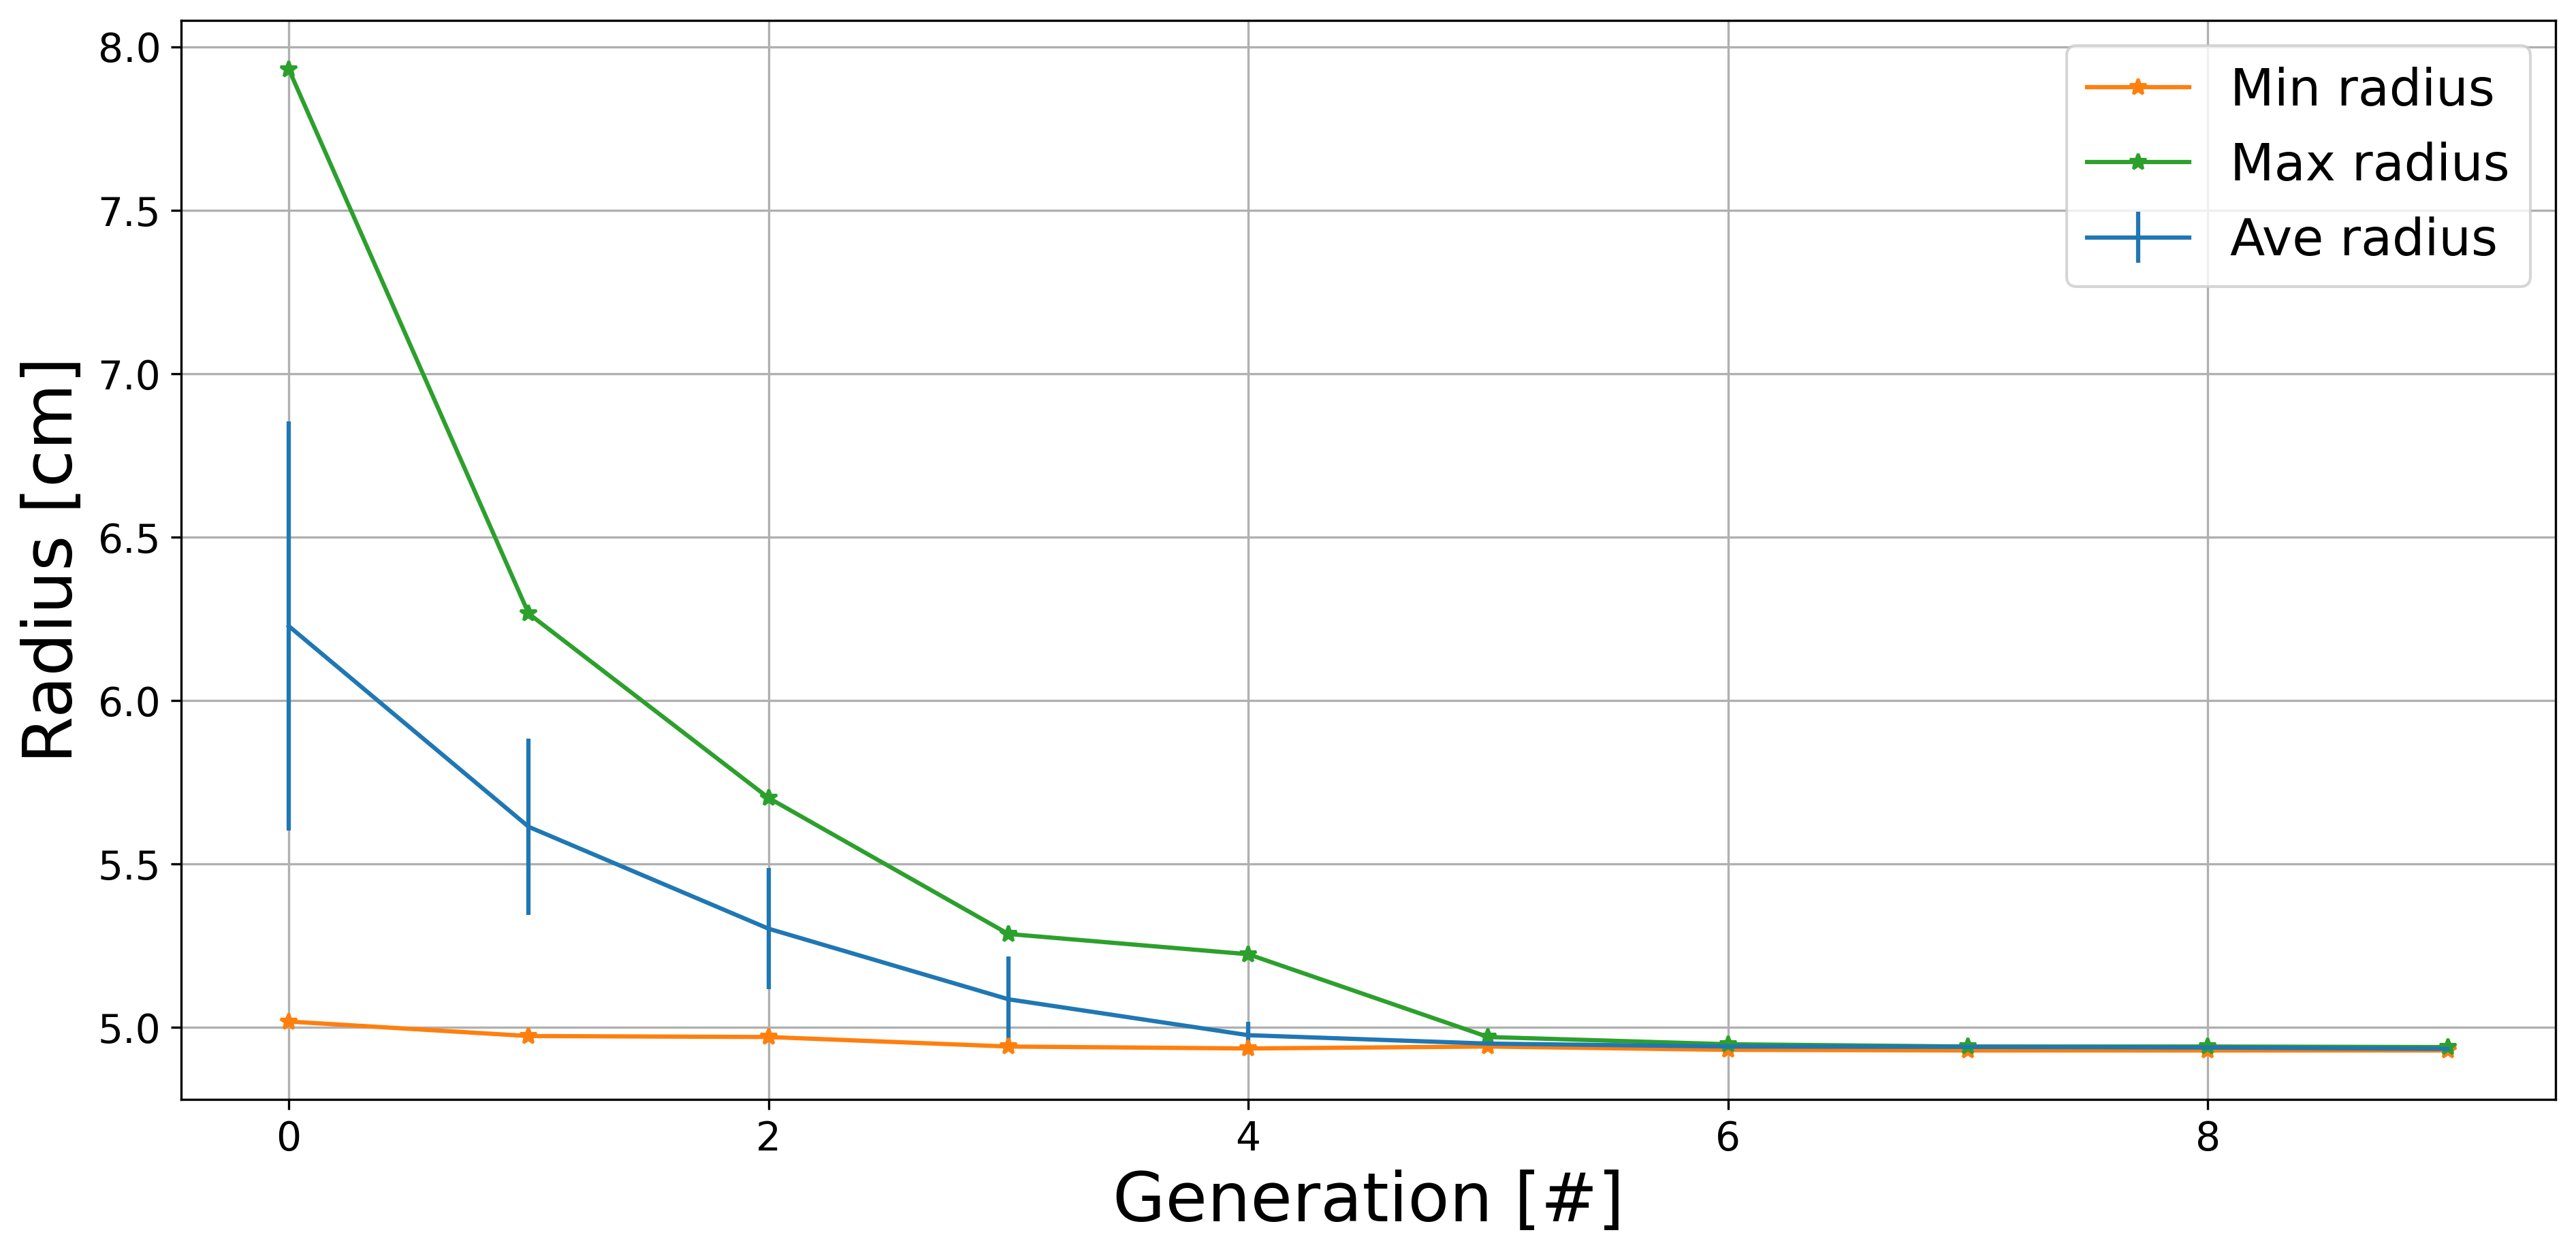
\includegraphics[width=0.85\linewidth]{../docs/figures/radius-convergence.png} 
        \caption{Results for each generation for \gls{ROLLO}'s genetic algorithm 
        optimization to the find the critical radius of a  $^{239}Pu$ bare sphere.}
    \end{figure}
    \textbf{ROLLO successfully finds the critical radius of the $^{239}Pu$ bare sphere 
    to be 4.9856cm.}
\end{frame}

\subsection{Optimization Methodology}
\begin{frame}
    \frametitle{AHTR Optimization Problem Definitions}
    \begin{block}{Varied Input Parameters}
        \begin{itemize}
            \item TRISO fuel packing fraction fraction distribution 
            \item Total fuel packing fraction 
            \item Coolant channel shape 
        \end{itemize}
    \end{block}
    \begin{block}{AHTR Optimization Objectives}
        \begin{figure}
            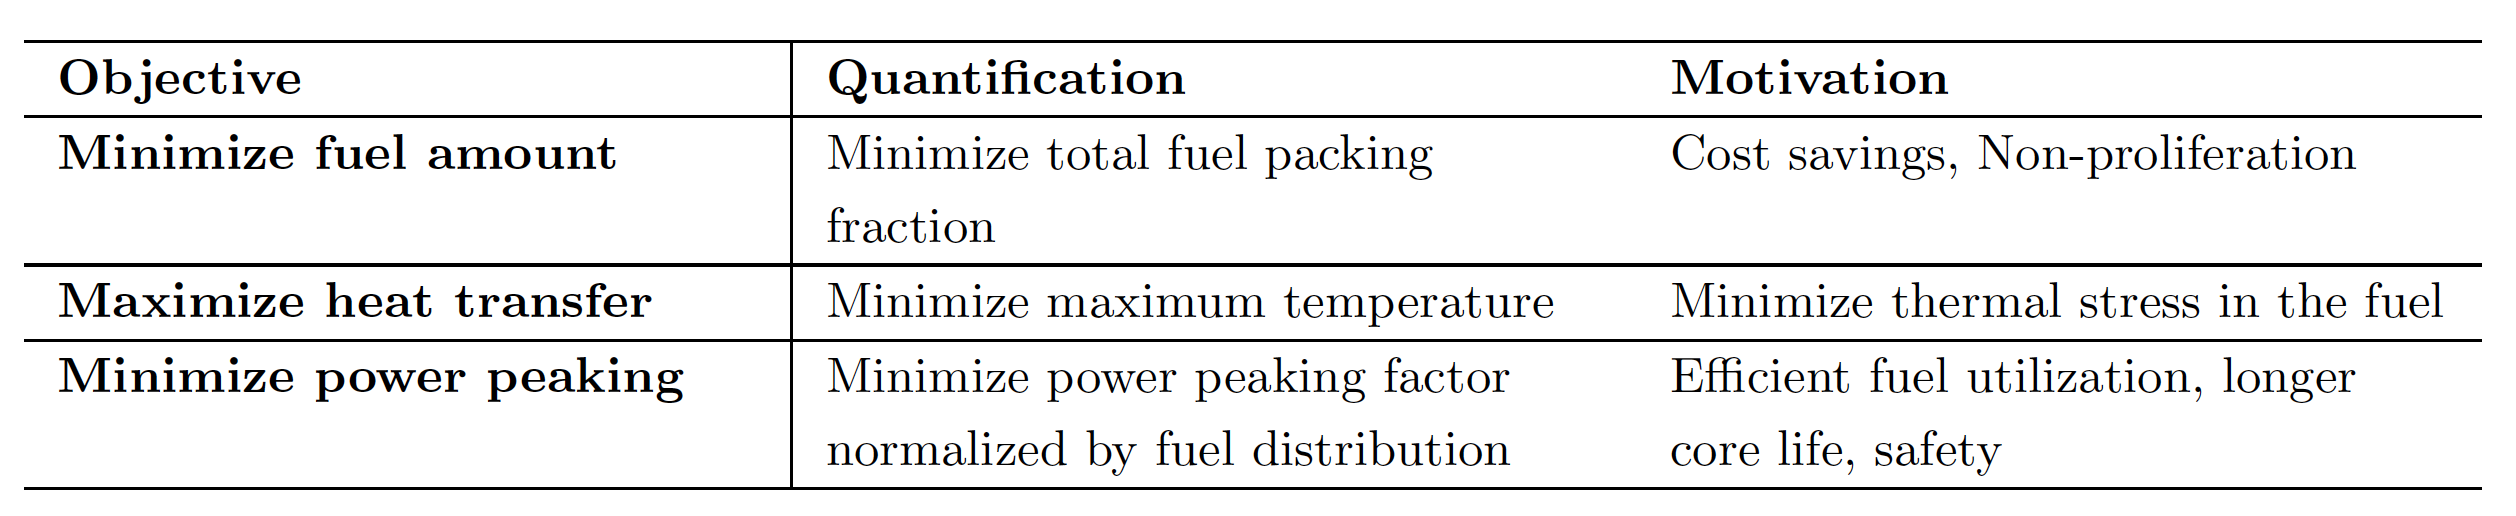
\includegraphics[width=0.9\linewidth]{figures/ahtr-opt-obj.png} 
            \caption{Optimization problem objectives.}
        \end{figure}
    \end{block}
\end{frame}

\begin{frame}
    \frametitle{AHTR Geometries}
    \begin{figure}
        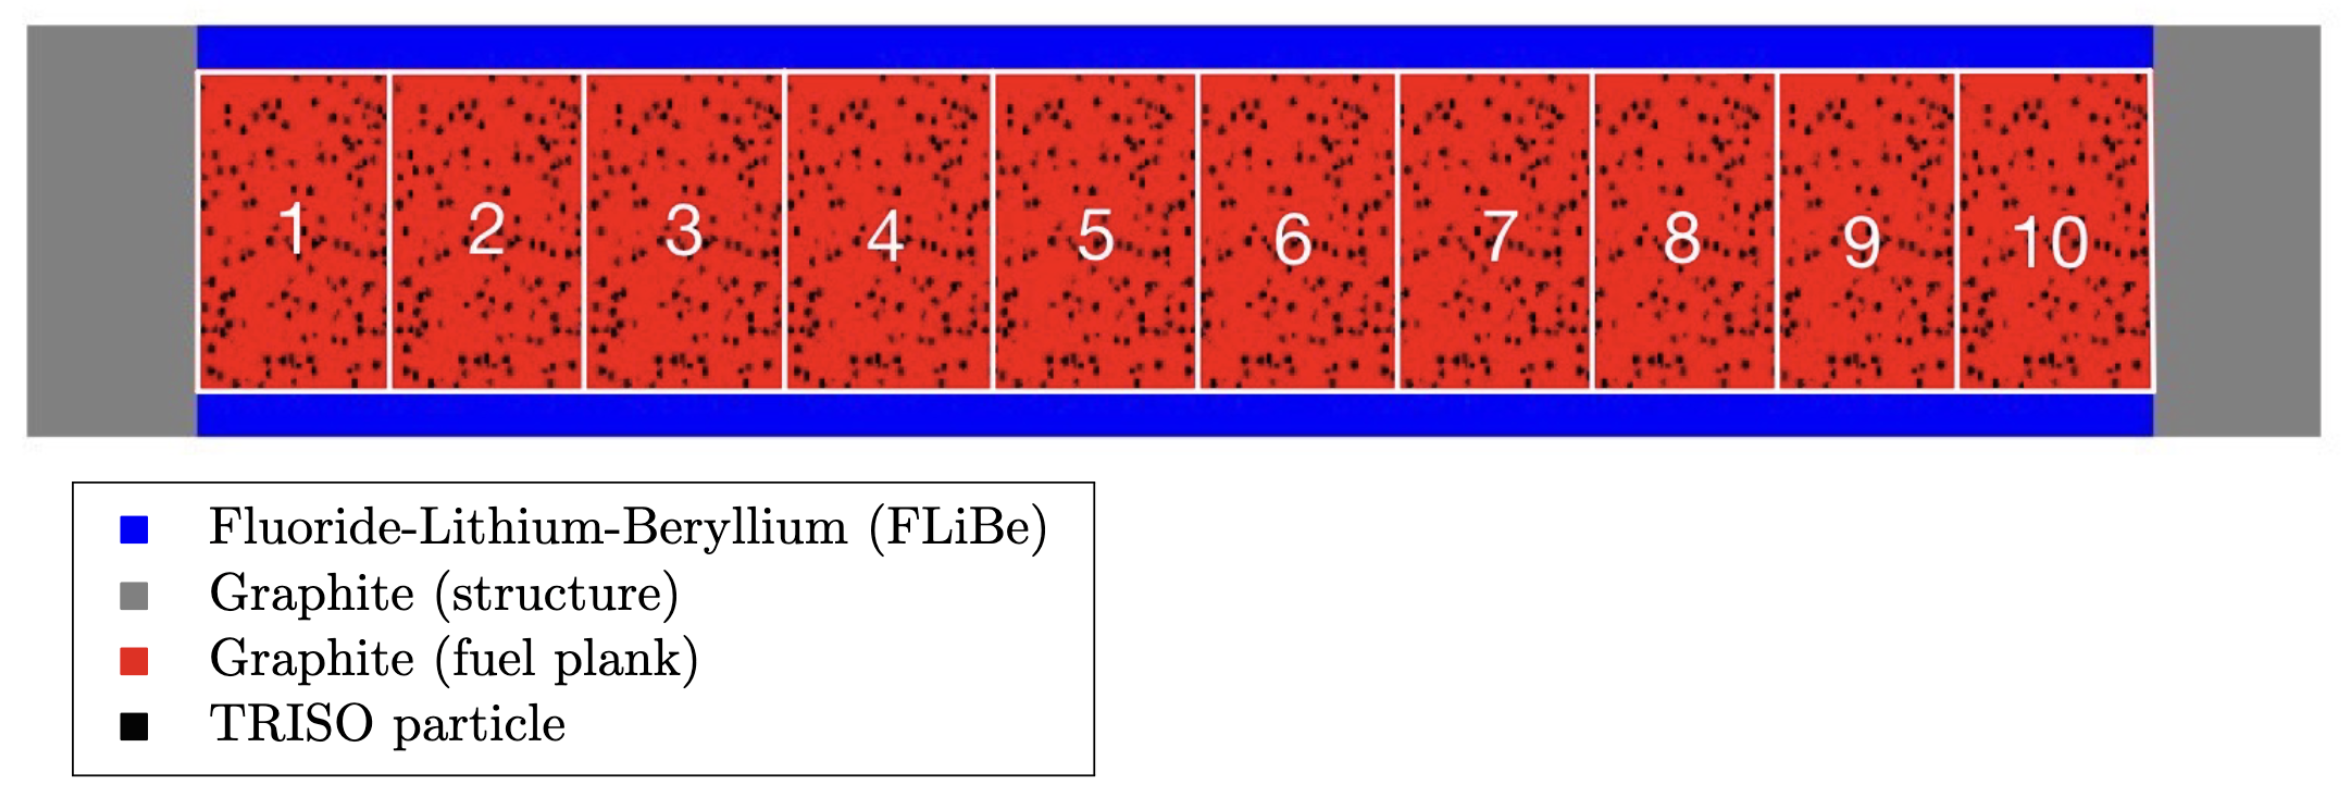
\includegraphics[width=0.9\linewidth]{figures/straightened-plank-pres.png} 
        \caption{AHTR Plank.}
    \end{figure}
\end{frame}

\begin{frame}
    \frametitle{AHTR Geometries}
    \begin{figure}
        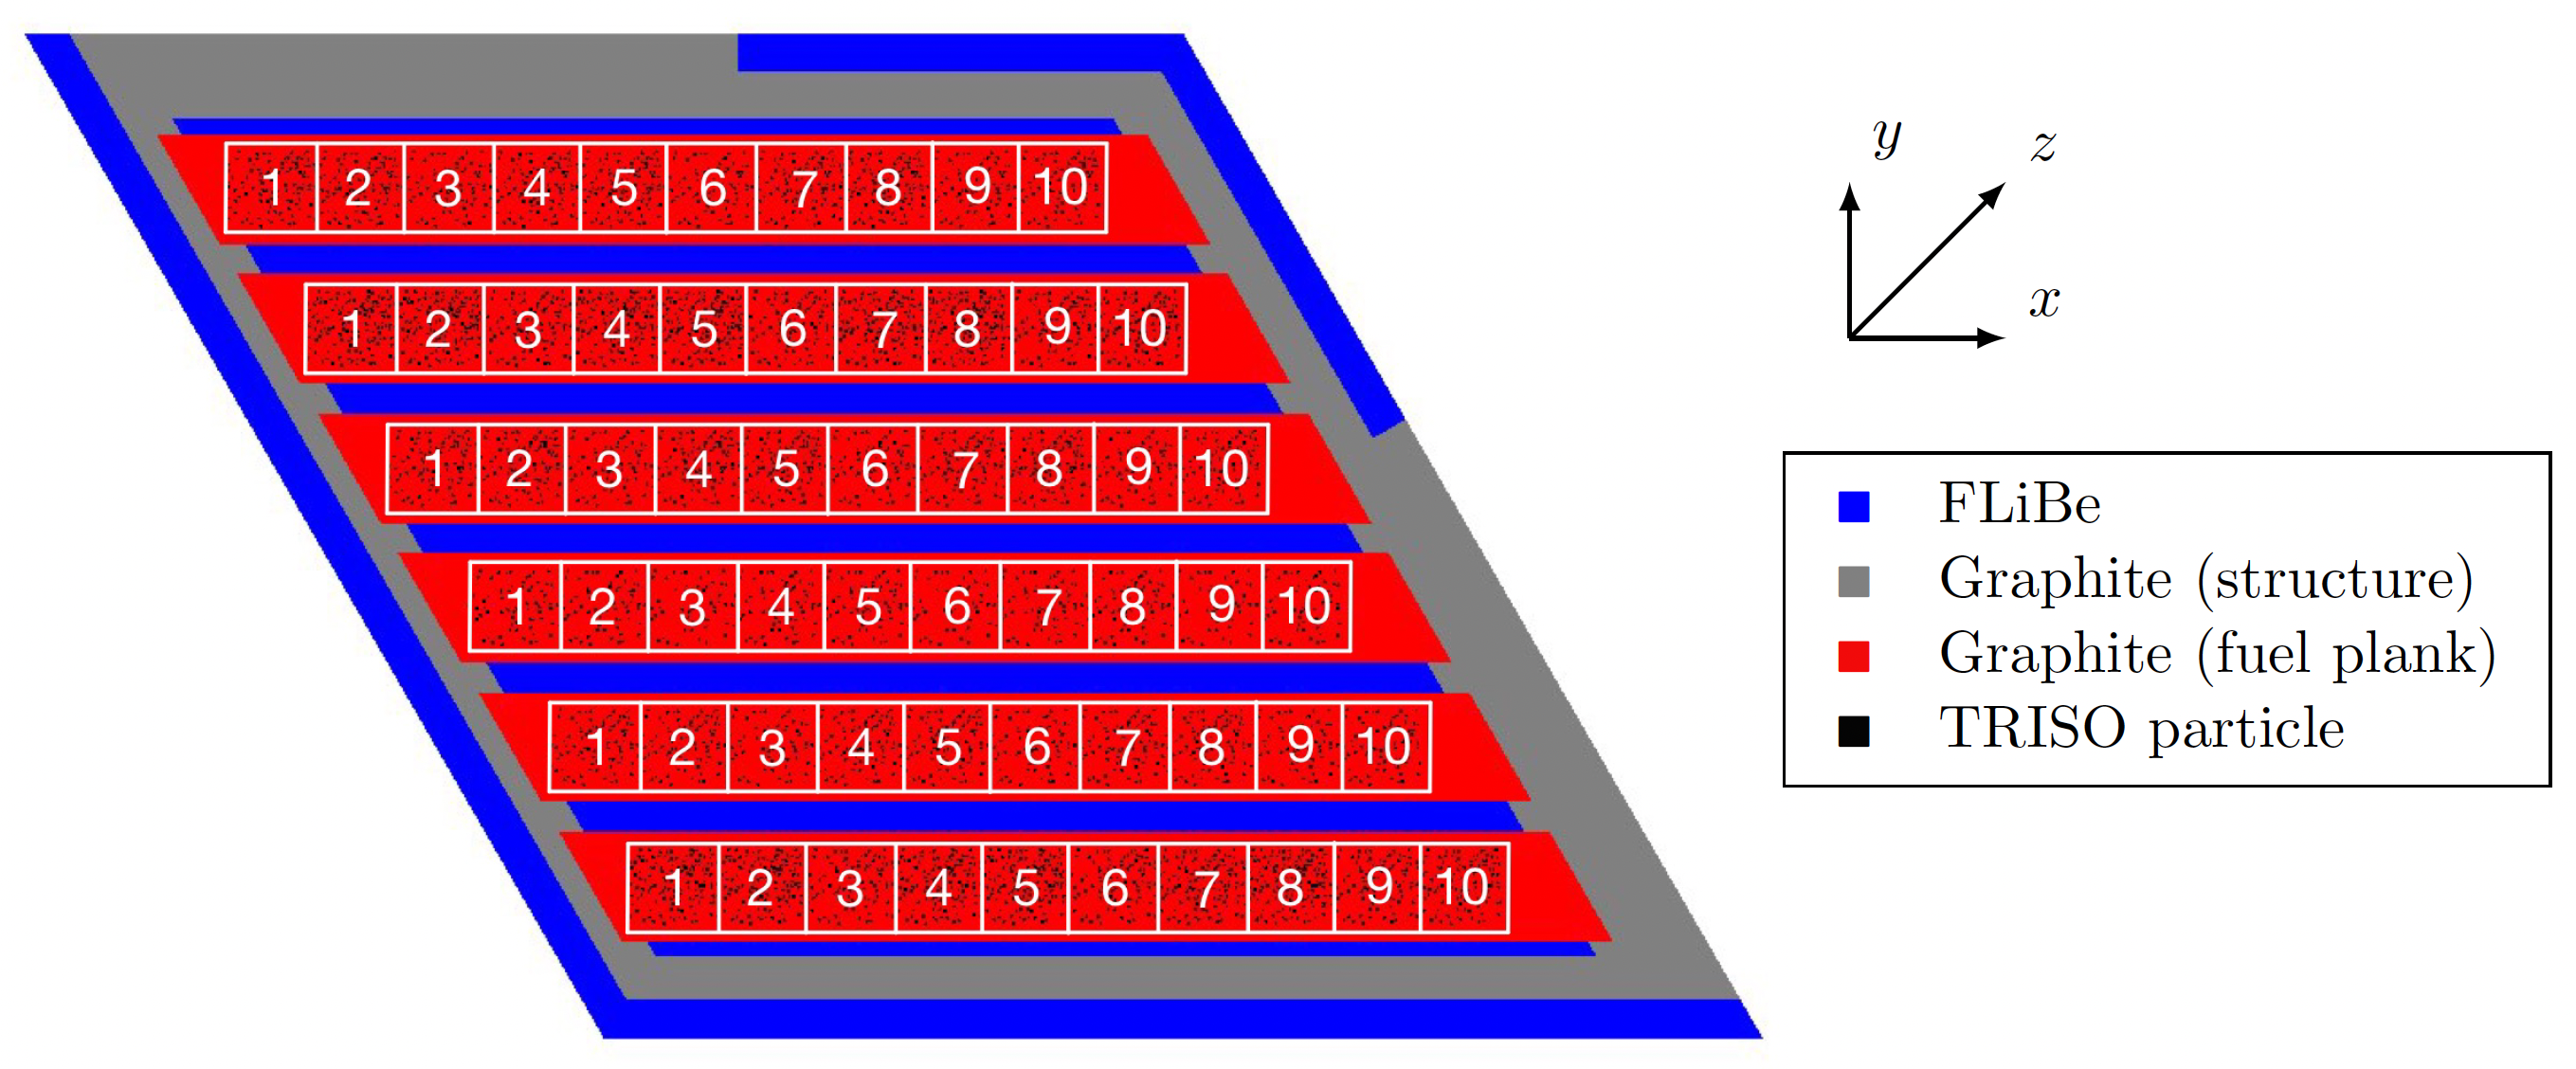
\includegraphics[width=0.9\linewidth]{figures/ahtr-assembly-pres.png} 
        \caption{AHTR One-Third Assembly.}
    \end{figure}
\end{frame}

\begin{frame}
    \frametitle{AHTR Modeling Workflow}
    \begin{figure}
        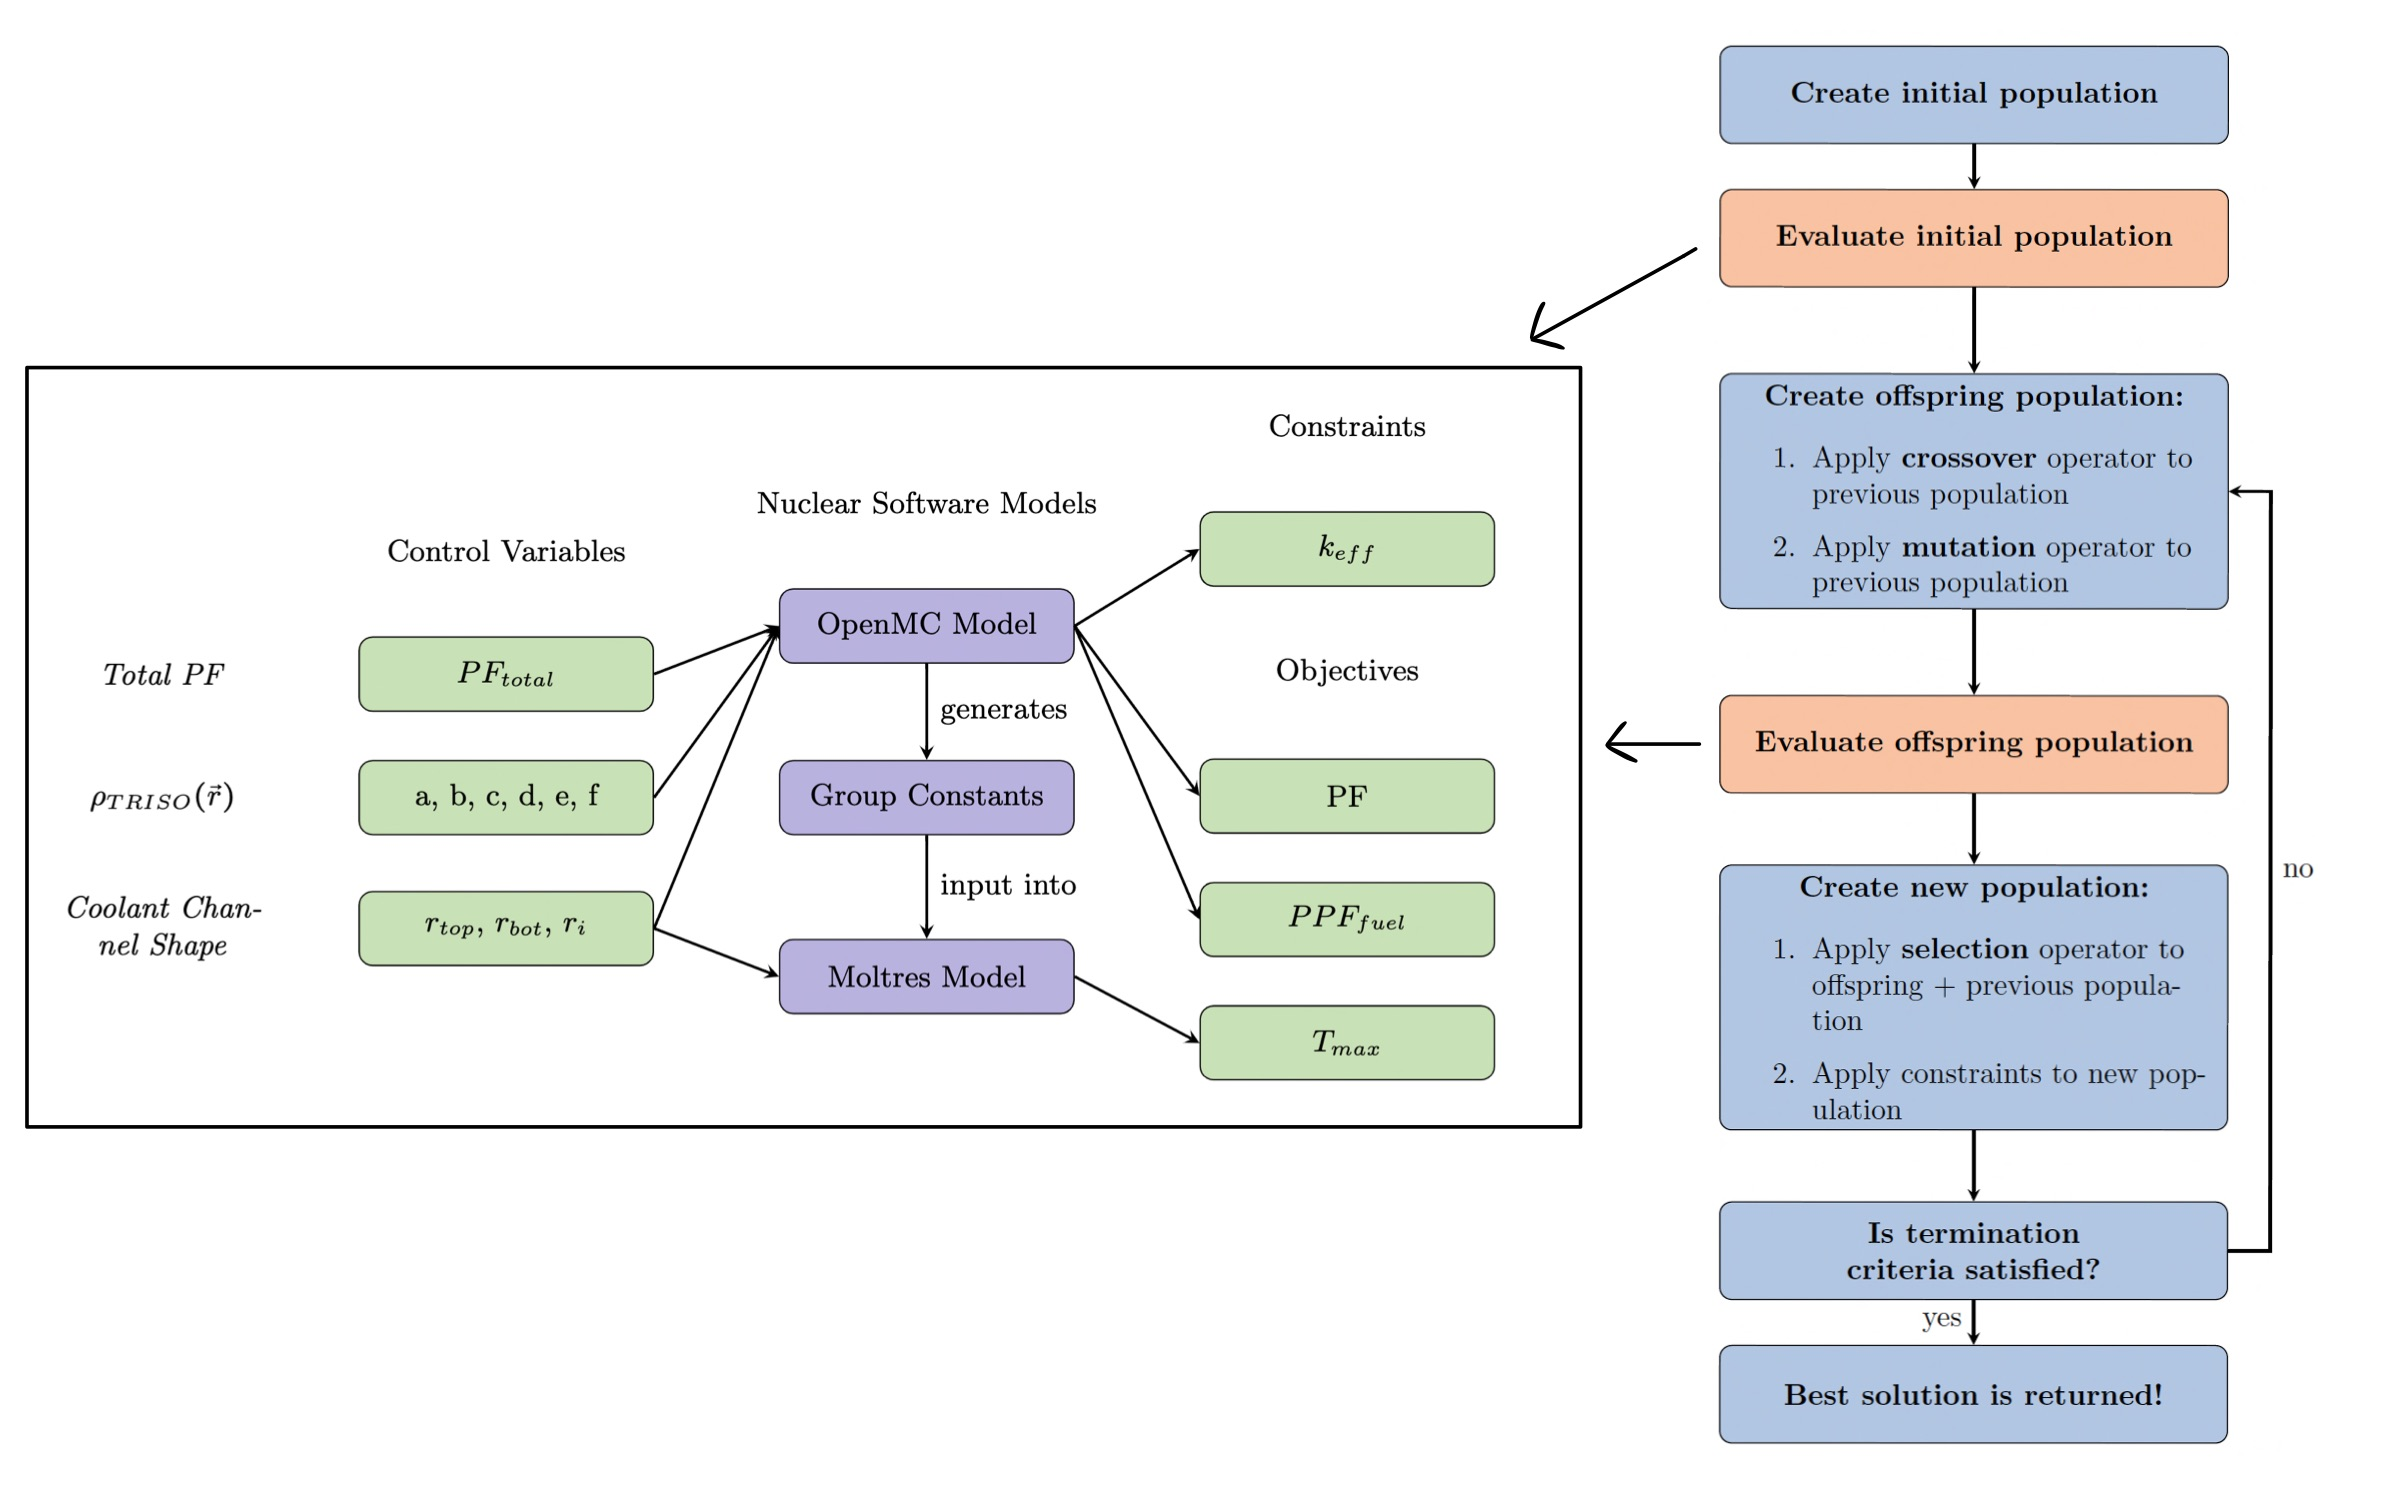
\includegraphics[width=0.9\linewidth]{figures/ahtr-modeling-workflow.png} 
        \caption{AHTR Modeling Workflow.}
    \end{figure}
\end{frame}

\subsection{AHTR Plank Optimization Results}

\subsection{AHTR One-Third Assembly Optimization Results}